\documentclass[10pt]{beamer}

\mode<presentation>
{
  \usetheme[height=1.25cm]{Madrid}
  \setbeamertemplate{navigation symbols}{}
  \setbeamercolor{alerted text}{fg=illini}
}

\usebackgroundtemplate{
\includegraphics[width=\paperwidth,height=\paperheight]{uc-background}}

\usepackage[english]{babel}
\usepackage{epsfig,subfigure,bm}
\usepackage{multimedia}
\usepackage{psfrag}
\usepackage{animate}

\usefonttheme{metropolis} % default family is serif
%%%%%% Begin of my macros and options

\setbeamertemplate{section in toc shaded}[default][55]
\setbeamertemplate{subsection in toc shaded}[default][55]
\setbeamercolor{block title}{fg=white,bg=illini}
\setbeamercolor{block body}{fg=black,bg=mygrey}

\setbeamercolor{emphprimary}{fg=CBlue}
\setbeamercolor{emphsecondary}{fg=illini}
\setbeamercolor{emphtertiary}{fg=mygreen}
\definecolor{darkForestGreen}{rgb}{.1,1,.1}
\definecolor{veryLightGray}{rgb}{.9,.9,.9}
\definecolor{greenApple}{rgb}{.3,.9,.3}

\setbeamercolor{frametitle}{bg=CBlue}   
\setbeamercolor{title}{bg=CBlue}

\usepackage{amsmath,amssymb,amsxtra,amsthm}
\usepackage{algorithm,algorithmic}
\usepackage{natbib}
\usepackage{bibentry}
\usepackage{xspace}
\usepackage{changepage}

\definecolor{myblue}{rgb}{.2,.2,.7}
\definecolor{myred}{rgb}{.7,.2,.2}
\definecolor{mygreen}{rgb}{.2,.7,.2}
\definecolor{mygrey}{rgb}{0.9,0.9,0.9}
\definecolor{CBlue}{cmyk}{1,0.25,0,0}
\definecolor{illini}{rgb}{0.98,0.4,0.05}
\definecolor{black}{cmyk}{0,0,0,1}

\newcommand{\myemph}[1]{{\usebeamercolor[fg]{emphprimary}
    \textbf{#1}}}
\newcommand{\myemphalt}[1]{{\usebeamercolor[fg]{emphsecondary}
    \textbf{#1}}}

\graphicspath{{figs/}}

\title[Math for Robotics] % (optional, use only with long paper titles)
{CSE276C - Integration of Functions}

\author[H.~I. Christensen] % (optional, use only with lots of authors)
{Henrik I.~Christensen}
% - Give the names in the same order as the appear in the paper.  -
% Use the \inst{?} command only if the authors have different
% affiliation.

\AtBeginSection[]
{
   \begin{frame}
       \frametitle{Outline}
       \tableofcontents[currentsection]
   \end{frame}
}

\institute[UCSD] % (optional, but mostly needed)
{
  \begin{minipage}[c]{.2\textwidth}
    
\includegraphics[width=.65\linewidth]{ucsealnew}%
  \end{minipage}%
  \begin{minipage}[c]{.6\textwidth}
    \small
%%    \begin{center}
      Computer Science and Engineering\\
      University of California, San Diego\\
      \myemph{\url{http://cri.ucsd.edu}}\\          
%%    \end{center}

  \end{minipage}
%%  \vspace*{1ex}
}
%% - Use the \inst command only if there are several affiliations.
%% - Keep it simple, no one is interested in your street address.

\bigskip

\date[Oct 2020]% (optional, should be abbreviation of conference name)
{\small%
  October 2020}

\begin{document}
  
\nobibliography{/Users/hic/Dropbox/bibliography/bib-file}
\bibliographystyle{plain}

\begin{frame}[plain]
  \titlepage
\end{frame}

\begin{frame}
  \frametitle{Introduction}
  \begin{itemize}
  \item Interested in integration of function to allow estimation of
    future value
  \item Lots of potential applications in robotics
    \begin{itemize}
    \item Position estimation
    \item Path optimization
    \item Image restoration
    \end{itemize}
  \item Consider both end-point and boundary value problems, which
    anchors the problem
  \end{itemize}
\end{frame}

\begin{frame}
  \frametitle{Introduction - Setting the stage}
  \begin{itemize}
  \item We are trying to solve
    \[
      I = \int_a^b f(x) dx
    \]
    \item trying to solve I = y(b) for the equation
    \[
      \frac{\partial y}{\partial x} = f(x)
    \] 
  \item with the boundary condition
    \[
      y(a) = 0
    \]
  \item Objective to generate a good estimate of y(b) with a
    reasonable number of evaluations
  \item Emphasis on 1D problems, but in most cases generalization is
    straight forward
  \end{itemize}
\end{frame}

\begin{frame}
  \frametitle{Setting the stage}
  \centerline{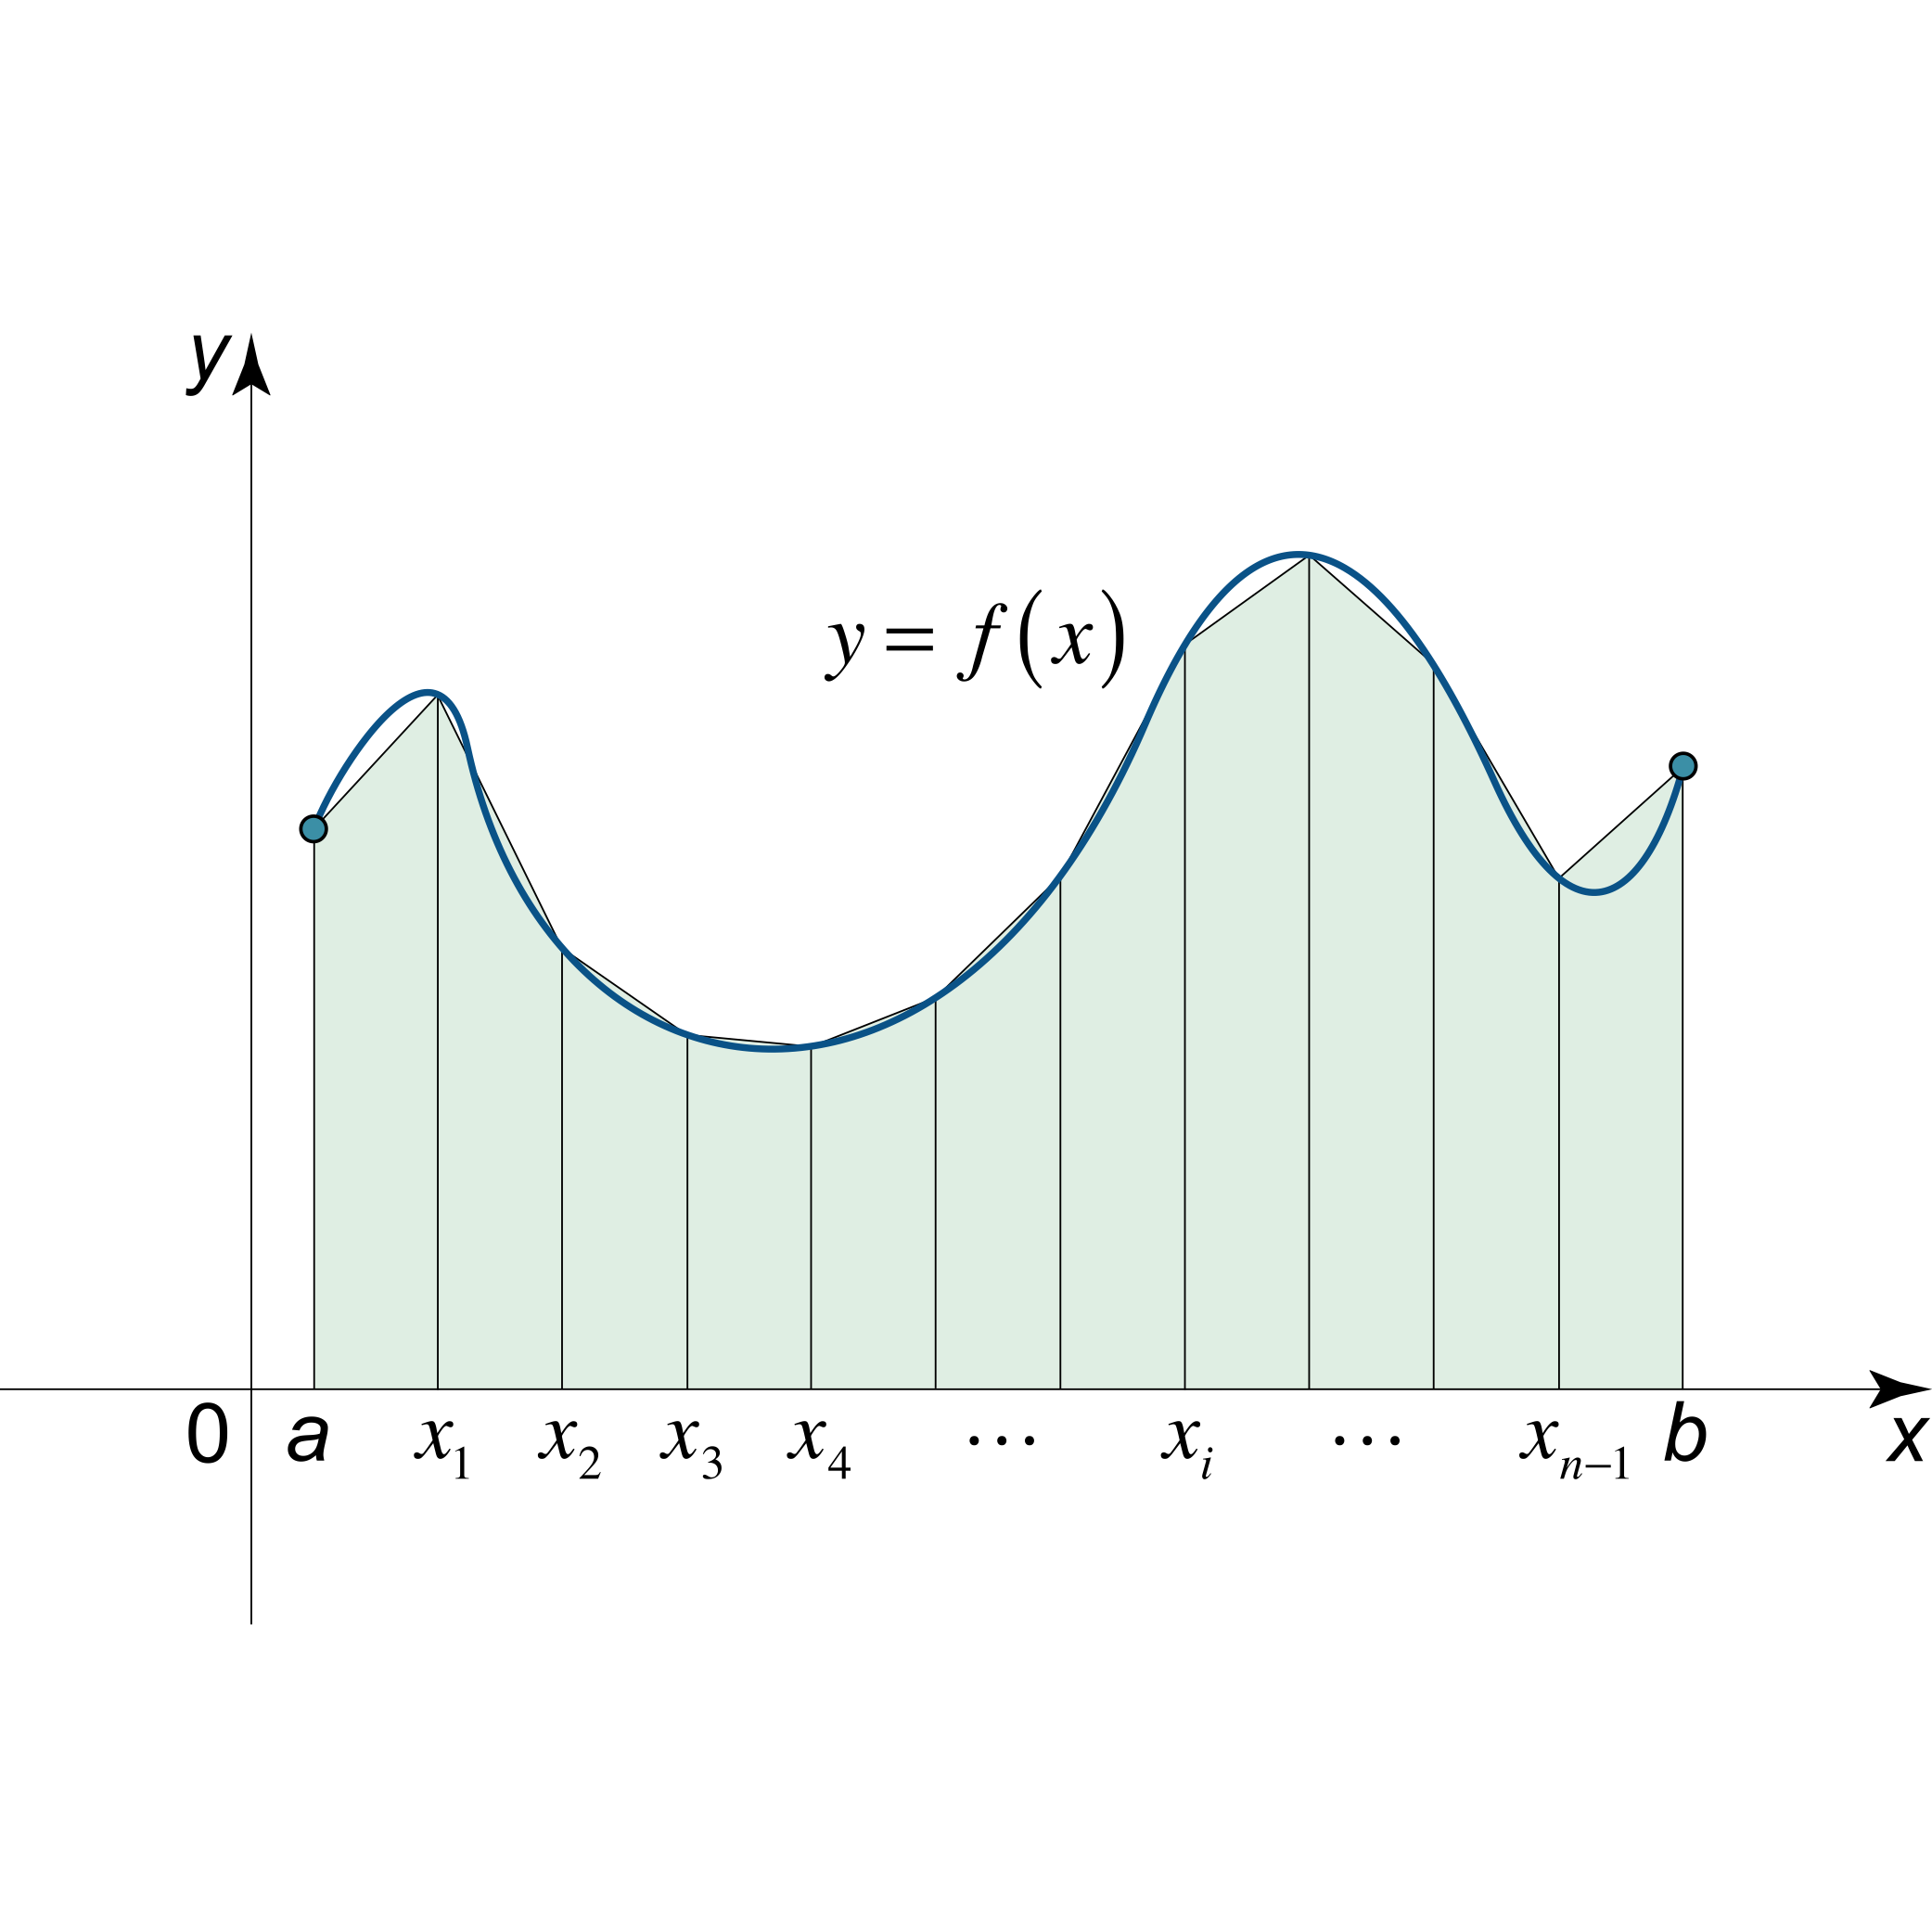
\includegraphics[height=7cm]{trapezoid}}
\end{frame}

\begin{frame}
  \frametitle{Basic use of Simpson's rule}
  \begin{itemize}
  \item Consider equally spaces data points
    \[
      x_i = x_0 + i h \mbox{ ~~~~~~~~} i = 0, 1, ..., N
    \]
    
  \item the function is evaluated at $x_i$
    \[
      f_i = f(x_i)
    \]
  \item The Newton-Cotes rules is then
    \[
      \int_{x_0}^{x_1} f(x) dx = \frac{f_1+f_0}{2} h + O(f'' h^3)
    \]
  \item The Simpson rules is
    \[
      \int_{x_0}^{x_2} f(x) dx = \frac{h}{3} (f_0 + 4 f_1 + f_2) + O(h^5 f^{(4)})
    \]
  \item which is exact to the 3rd degree
  \item The Simpson $\frac{3}{8}$ rule
    \[
      \int_{x_0}^{x_3} f(x) dx = \frac{h}{8} (3 f_0 + 9 f_1 + 9 f_2 + 3 f_3)
    \]
  \item There are a series of rules for higher order, check literature
  \end{itemize}
\end{frame}


\begin{frame}
  \frametitle{Simpson's Rule}
  \centerline{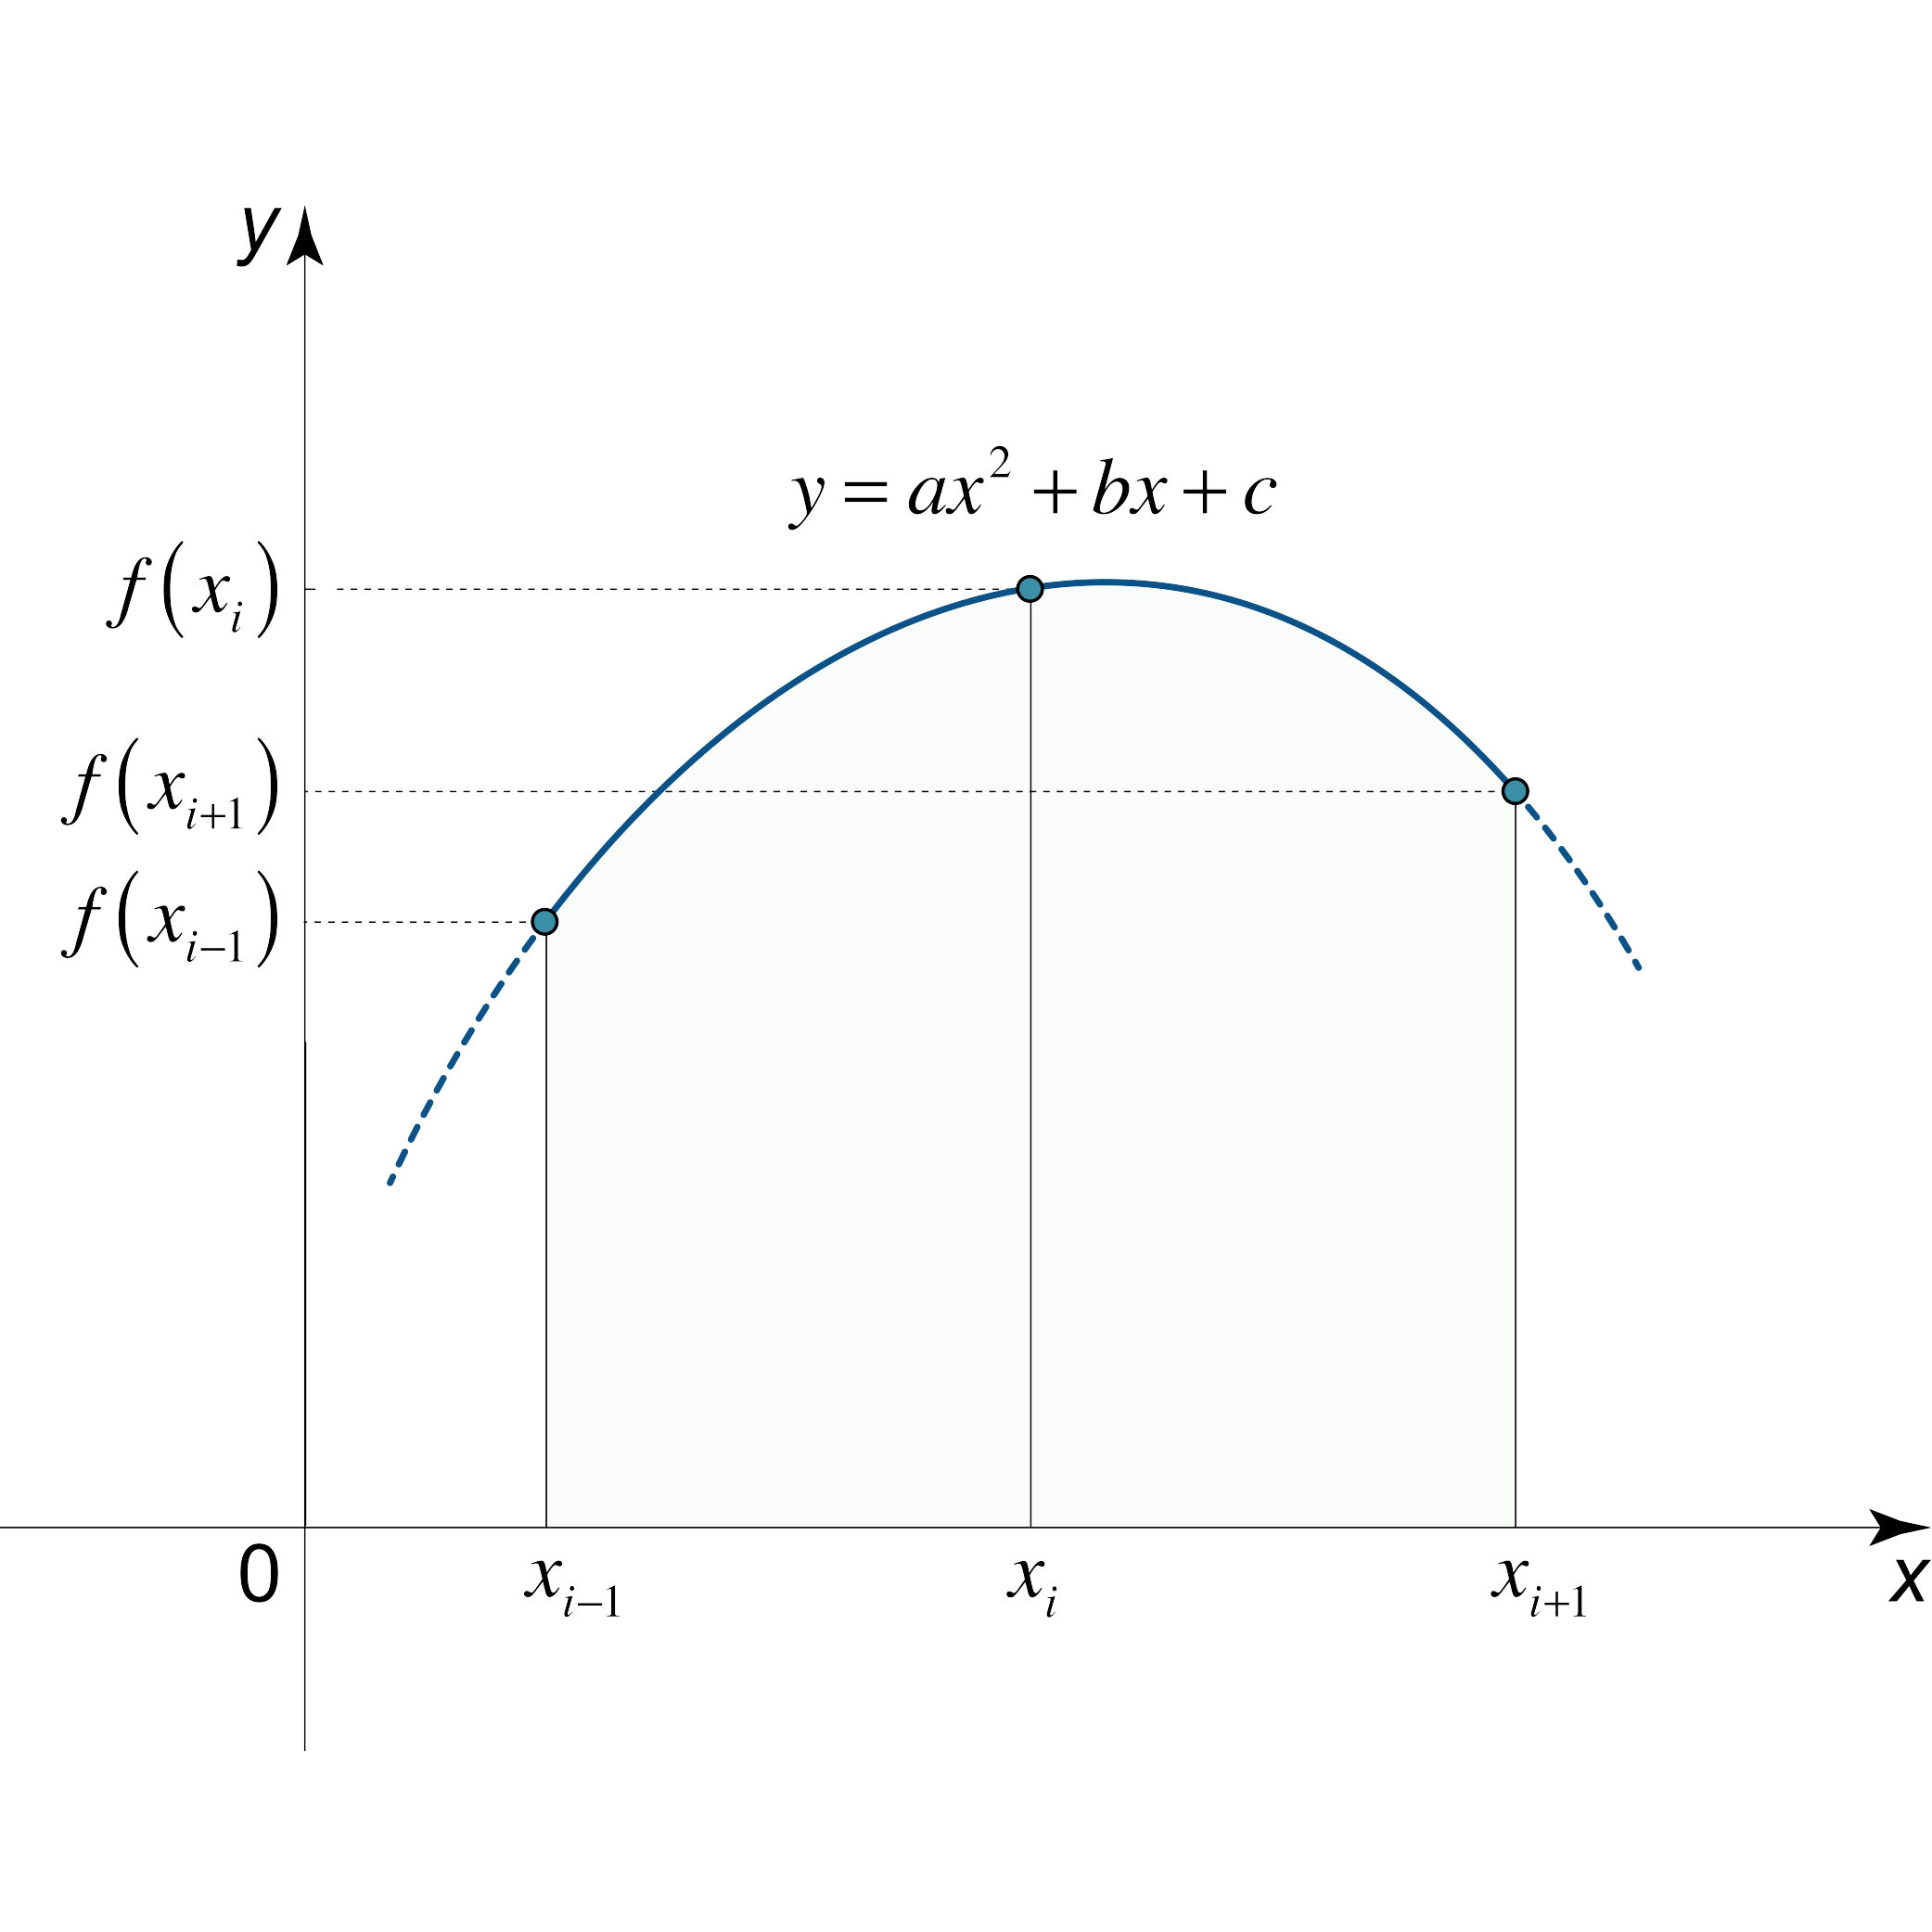
\includegraphics[height=7cm]{simpsons-rule}}
\end{frame}

\begin{frame}
  \frametitle{Simpson / Trapezoid Rules}
  \begin{itemize}
  \item Clearly the local rules can be chained into a longer evaluation
  \item $(x_0, x_1), (x_1, x_2), \ldots, (x_{N-1},x_N)$ to get an extended
    trapezoid form
    \[
      \int_{x_0}^{x_N} f(x) dx = h(\frac{1}{2} f_0 + f_1 + f_2 + \ldots + f_{N-1} + \frac{1}{2} f_N )
    \]
  \item The error estimate is
    \[
      O\left( \frac{(x_N - x_0) f''}{N^2} \right)
    \]
  \end{itemize}
\end{frame}

\begin{frame}
  \frametitle{Trapezoid Rule - Strategy?}
  \begin{itemize}
  \item How can you effective use the trapezoid rule?
    \pause
  \item Use of a coarse to fine strategy and watch convergence
  \item This is termed Romberg integration in numerical toolboxes
  \item In general these methods generate good accuracy for proper functions? 
  \end{itemize}
\end{frame}

\begin{frame}
  \frametitle{Handling of improper function}
  \begin{itemize}
  \item What is an improper function?
    \pause
    \begin{enumerate}
    \item Integrand goes to a finite value but cannot be evaluated at a point, such as
      \[
        \frac{sin x}{x} \mbox{ ~~~ at ~~~ } x=0
      \]
    \item Upper limit is $\infty$ or lower limit is $-\infty$
    \item Has a singularity at a boundary point, e.g.,
      \[
        x^{-1/2} \mbox{~~~~ at ~~~~~} x = 0
      \]
    \item Has a singularity within the interval at a known location
    \item Has a singularity within the interval at an unknown location
    \end{enumerate}
  \item If the value is infinite, e.g.,
    \[
      \int_0^{\infty} x^{-1} dx \mbox{~~~~or~~~~} \int_{-\infty}^{\infty} cos x dx
    \] it is not improper but impossible
  \end{itemize}
\end{frame}

\begin{frame}
  \frametitle{The Euler-Maclaurin Summation Formula}
  \begin{itemize}
  \item We can write the basic Simpson's rule as
    \[
      \begin{array}{rcl}
      \int_a^b f(x) dx &=& \frac{h}{2} \left[ f(a) + 2 \sum_{k=1}^{N-1} f (a + kh) + f(b) \right]\\
                       && - \sum_{k=1}^{N/2} \frac{h^{2k} B_{2k}}{(2k)!}[ f^{(2k-1)}(b) - f^{(2k-1)}(a)] \\
                       && - \sum_{k=0}^{N-1} \frac{h^{2k+1} B_{2k}}{(2k)!} f^{(2k)}(a + kh + \theta h) \\
      \end{array}
    \]
  \item where 2m first derivatives are continuous over (a,b). h = (a-b)/N and $\theta\in(0,1)$
  \item So what are the B's?
  \item They are Bernoulli numbers
    \[
      \frac{t}{e^t-1} = \sum_{n=0}^{\infty} B_n \frac{t^n}{n!}
    \]
  \item example values
    \[
      \begin{array}{rcl}
        B_0 & = & 1\\
        B_2 & = & \frac{1}{6} \\
        B_4 & = & - \frac{1}{30}\\
      \end{array}
    \]
  \item Enables you to compute an estimate of the error for a particular integration
  \item Other integration functions have similar error functions - decreasing with complexity
  \end{itemize}
\end{frame}

\begin{frame}
  \frametitle{Extended Mid-point Formulation}
  \begin{itemize}
  \item In many cases using the mid-point is a valuable alternative
    \[
      \int_{x_0}^{x_{N-1}} f(x) dx = h (f_{1/2} + f_{3/2} + \ldots + f_{N-3/2}) + O(\frac{1}{N^2})
    \]
  \item When combined with the Euler-Maclaurin you get
    \[
      \begin{array}{rcl}
        \int_{x_0}^{x_{N-1}} f(x) dx &=& h (f_{1/2} + f_{3/2} + \ldots + f_{N-3/2}) \\
                & + & \frac{B_2 h^2}{4} (f'_{N-1} - f'_0) + \ldots + \frac{B_{2k} h^{2k}}{(2k)!} (f^{(2k)}_{N-1} - f^{(2k)}_0) + \ldots \\
      \end{array}
    \]
  \item We can do this recursively to estimate convergence
  \end{itemize}
\end{frame}

\begin{frame}
  \frametitle{Handling improper integrals}
  \begin{itemize}
  \item A trick for improper integrals is to do variable substitution to eliminate a challenge
  \item Say one of the values is at $-\infty$ or $\infty$ we can substitute
    \[
      \int_a^b f(x) dx = \int_{1/b}^{1/a} \frac{1}{t^2} f\left( \frac{1}{t} \right) dt
    \]
  \end{itemize}
\end{frame}

\begin{frame}
  \frametitle{Variable substitution}
  \begin{itemize}
  \item More generally we can do variable substitution as
    \[
      I = \int_a^b f(x) dx = \int_c^d f(x(t)) \frac{dx}{dt} dt
    \]
  \item An example is the Schwartz $\tanh$ rule
    \[
      x = \frac{1}{2} (b+a) + \frac{1}{2} (b-a) \tanh(t) \mbox{~~~ } x\in[a,b] \mbox{ and } t\in[-\infty,\infty]
    \]
  \item where
    \[
      \frac{\partial x}{\partial t} = \frac{1}{2} (b-a) sech^2(t) = \frac{2}{b-a} (b-t) (t-a)
    \]
  \item $sech()$ converges very rapidly for $t\rightarrow \infty$ which allows for integration close to singularities
  \end{itemize}
\end{frame}

\begin{frame}
  \frametitle{Gauss Integration}
  \begin{itemize}
  \item Sometimes uniform sampling is not ideal
  \item A Gauss model may be an alternative
  \item The idea is
    \[
      \int_a^b W(x) f(x) dx \approx \sum_{j=0}^{N-1} W_j f(x_j)
    \]
  \item For polynomials this can be an exact approximation
  \item We can approximate f(x) with a Gaussian Mixture and choose weights to match
    \[
      f(x) \approx \sum_{k=0}^N W_k N(x | x_k, \sigma_k)
    \]
  \end{itemize}
\end{frame}

\begin{frame}
  \frametitle{Partitioned / Adaptive Integration}
  \begin{itemize}
  \item If you have a function with variable dynamics it makes sense
    to partition the integration into intervals and use Romberg
    integration on each interval, i.e.
    \[
      \begin{array}{rcl}
        I & = & \int_a^b f(x) dx \\
          & = & \int_a^m f(x) dx + \int_m^b f(x) dx\\
      \end{array}
    \]
  \item Rule 1 of data analysis understand your data     
  \end{itemize}
\end{frame}

\begin{frame}
  \frametitle{Summary}
  \begin{itemize}
  \item Simple linear approximations are effective for well-behaved functions
  \item The order of your approximation can vary according to function complexity
  \item Using Bernoulli functions we can approximate the estimated error
  \item Recursive estimation with error monitoring is often effective
  \item Do a function analysis first to make sure function is proper
  \item Next time we will discuss integration of ODE with standard
    methods such as Runga-Kutta, Step-size variation, etc.
  \end{itemize}
\end{frame}
\begin{frame}
  \frametitle{Questions}
  \centerline{\Huge Questions}
\end{frame}

\end{document}

%%% Local Variables:
%%% mode: latex
%%% TeX-master: t
%%% End:
